% !TEX root = main.tex
\chapter{Airfoils and Inverted Wings}

Achieving a large negative lift coefficient $C_L$ can be done in many ways. Inspecting race cars throughout the years show that airfoils have been used as early as 1966 when Jim Hall attached a rear wing to his Chaparral 2E \cite{hucho}. Since then, the inverted wings have been a staple in the racing industry with various three dimensional geometries affecting the overall performance even further.

This chapter covers the pressure distribution of various airfoils, the selection criterions of the competition, three dimensional geometrical effects and the tools of the optimization trade.

\section{Airfoil theory}

  \begin{figure}
    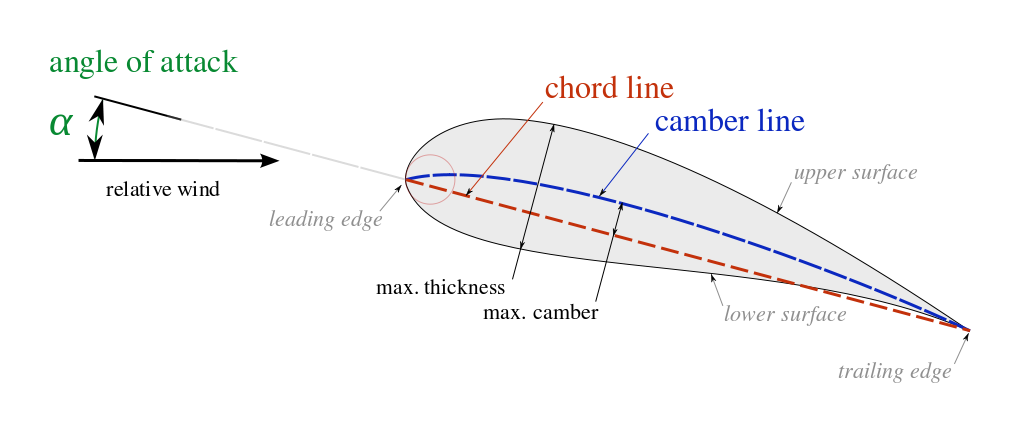
\includegraphics[width=\textwidth]{camberAOA}
    \caption{Figure explaining angle of attack, chord line, camber line, upper surface (suction surface), lower surface (pressure side), leading edge and trailing edge. Figure taken from \cite{wikicamberAOA}.}
    \label{fig:camberAOA}
  \end{figure}

  An airfoil is the 2-dimensional cross section of a wing, that is defining of the wing's lifting characteristics. It is important to know the nomenclature, which is shown on figure \ref{fig:camberAOA}: The leading edge is  the most forward point of the wing, the trailing edge is the most rearward point of the wing. Camber is how much the wing the wing \emph{bends}.

  \begin{figure}
    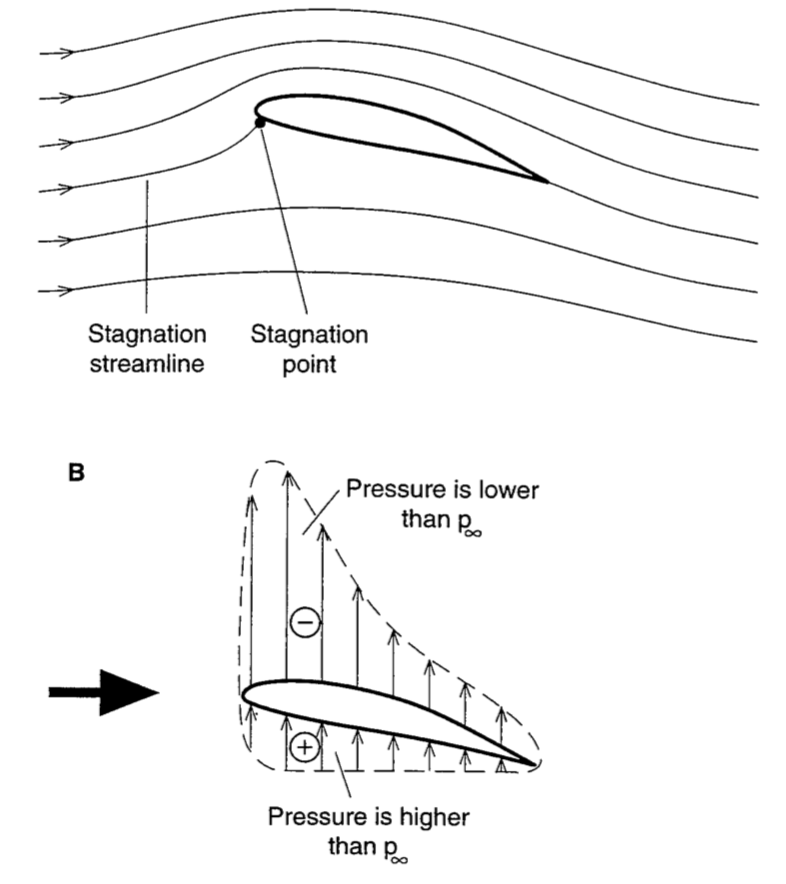
\includegraphics[width=\textwidth]{airfoilstreamlines}
    \caption{A figure showing the streamlines around a slightly cambered airfoil, along with its pressure distribution below. Figure taken from \cite{jkatz}.}
    \label{fig:airfoilstreamlines}
  \end{figure}

  When an airfoil moves in a fluid, the streamlines of the particles move as seen in figure \ref{fig:airfoilstreamlines}. The streamline stops at the stagnation point, which is usually the leading edge. The other can be divided into two categories, as the flow can only go to two places: The \emph{suction surface} and the \emph{pressure surface}.

  The suction surface is the surface where the flow accelerates to high velocities and the pressure drops. This can be seen on the top part of figure \ref{fig:airfoilstreamlines}, where the corresponding pressure distribution can be seen below as the (-) part. A peak of very low pressure can be found near the leading edge, which is often called the suction peak.

  The pressure surface is the surface where the flow decellerates to lower velocities and the pressure increases. This is the bottom part of \ref{fig:airfoilstreamlines}, which provides a much lower force from the pressure than the suction side.

  The resulting changes in pressure forces the wing upwards, creating lift. It it important to note, that the suction side contributes considerably more to lift in most cases \cite{jkatz}.

  \subsection{Airfoil Lift and How to Increase it}

    Increasing the lifting capabilities of an airfoil can be done in several ways.

    First, the angle of attack of air airfoil usually increases lifting characteristics of a wing, until reaching a certain threshold where it falls off. An airfoil carries its lifting abilities usually while flow is attached - that is, where the streamlines follow the shape of the airfoil. If the flow separates from the surface of the airfoil, the lift behaviour becomes unpredictable. This effect is called \emph{stalling}.

    There are two types of stalling: Leading edge separation which are quite abrupt and greatly decreases lift, and trailing edge separation, which gradually reduces the lift. These are called a hard and soft stall, respectively. Thus, a soft stall is prefered in racing, as a hard stall will instantly change the car's handling abilities.

    Secondly, another way of changing the lift is by creating an effective change in angle of attack: Changing the wing's camber. The trailing edge of an airfoil's camberline is the largest contributor to lift. By changing the camber geometry, the lift can be changed greatly, and the largest increase is found in the trailing edge region. This is why the introduction of flaps is prominent in both aircraft and race car wings.

    Lastly, the thickness of the airfoil affects lift up to a certain point, and the optimum thickness is about $12\%$ of the camber length. For the interested ready, reference \cite{jkatz} explores this further.

  \subsection{Reynolds Number, Lift and Drag Coefficient}

    The Reynolds number is an dimensionless number that is used to predict the flow of fluids in different flow configurations. In general the Reynolds number is used to predict if a flow is laminar or turbulent. The Reynolds number is defined as:

    \begin{align}
      Re \equiv \frac{u_{\infty}L}{\nu},
      \intertext{where $\infty$ is the velocity of the fluid, $L$ is the characteristic Length, for an airfoil this would typically be the chord, and $\nu$ is the kinematic viscosity of the fluid.} \label{eq:ReynoldsNumber}
    \end{align}

    The usage of Reynolds number when designing an airfoil is the fact that the flow is similar for different scales of the same model if the Reynolds number is the same. Thereby a smaller model can be built and tested at a higher velocity that the full scale, thereby amounting to the same Reynolds number and fluid flow characteristics. \fxnote{When is it turbulent, when is it laminar? says so in jkatz}

    The lift coefficient is a dimensionless coefficient that relates the lift generated to the fluid the airfoil moves in, the velocity of the fluid and the reference area. This coefficient is defined as:

    \begin{align}
        C_l &\equiv \frac{F_l}{\frac{1}{2} \rho {u_\infty}^2 c}
        \intertext{Where $F_l$ is the lift per unit width, $\rho$ is the density of the fluid, $\dot{x_\infty}$ is the velocity of the surrounding fluid and $c$ is the chord length. For a specific wing, that is, where an airfoil has a physical extension, the lift coefficient is defined as:}
        C_L &\equiv \frac{F_L}{\frac{1}{2} \rho {u_\infty}^2 A}
        \intertext{Where $F_L$ is the total lift force, and $A$ is the surface area. For a wing with both camber and angle of attack, $C_L$ is found by the following formula:}
        C_L &= C_{L_\alpha} (\alpha + \alpha_{L_0})\label{eq:CL}
        \intertext{where $\alpha$ is the lift per angle of attack in radians, $\alpha_{L_0}$ is the airfoil's camber, which acts as a additional angle of attack effect, also in radians. $C_{L_\alpha}$ is given by \cite{nasalift}:}
        C_{L_\alpha} &= \frac{2\pi}{1+\frac{2}{\AR}} \label{eq:liftperAR}
    \end{align}
    However, it is important to note that equation \ref{eq:liftperAR} is derived for elliptical wings and is thus an approximation \cite{jkatz2}.

    Like lift, a dimensionless drag coefficient exist, that describes how drag is generated in a similar fashion:

    \begin{align}
      C_d &\equiv \frac{2F_d}{\rho {u}^2 A}
      \intertext{Where $F_d$ is the viscous drag force - the component of the force that is parallel with the flow velocity \cite{nasadrag}. The induced drag created by the lifting force must also be added in order to find the total drag coefficient \cite{nasainduceddrag}:}
      C_D &= C_d + C_{d_\text{induced}}\\
      \intertext{where $C_{d_\text{induced}}$ is given by:}
      C_{d_\text{induced}} &= \frac{C_L^2}{\epsilon \pi \AR }
    \end{align}
    The derivation and explanation hereof is found in the section below.

  \subsection{Aspect Ratio and End Plates}
  \label{subsec:endplates}

    An important identifyer when describing an actual finite wing is, apart from chord length and airfoil design, the width. The definition used for describing the physical span is called Aspect Ratio, and for a rectangular wing is:
    \begin{align}
        \AR_\text{actual} &= \frac{b}{c}
        \label{eq:ARactual}
    \end{align}
    Where $b$ is the width of the wing and $c$ is the chord length.

    \begin{figure}
      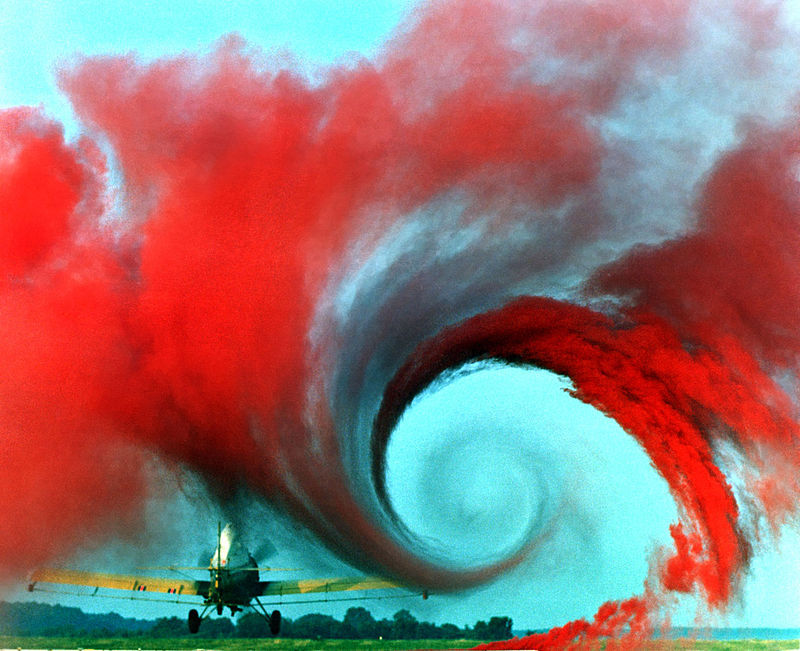
\includegraphics[width=\textwidth]{trailingtipvortex}
      \caption{The trailing tip vortex is clearly seen to the right. Thanks to the NASA's Wake Vortex Study for the photo \cite{nasatipvortex}.}
      \label{fig:trailingtipvortices}
    \end{figure}

    The effect of having a finite length is very important in race aerodynamics. As pressure is lowered and increased on the different sides, air is going to travel around the edge of the wing in a rolling motion. This creates a vortex, which is shown in figure \ref{fig:trailingtipvortices}. The phenomenon is called tip vortices, and the magnitude of the vortex is proportional to the lift coefficient of the wing. The area these vortices cover is very large and for wings with a small span will greatly reduces the lifting powers.

    These vortices are created by an effect called \emph{downwash} when talking aeroplanes. As the wing bends the air slightly downwards, it creates an opposite force due to Newton's second law which is lift. However, the sheet of air that passes over the length of the wing has a downward velocity component and will thus force air in that direction. This presses other air out of the way, allowing air above it to rush downwards to fill the gap. The same phenomenom is what happens at the edge of the wing, and again is what is shown in figure \ref{fig:trailingtipvortices}. When the wing \emph{bends} the airflow downward, drag is induced. While drag is almost negligible in our case, it is never wanted \cite{peterkampf}. For an elliptical wing, the induced drag coefficient is given by:

    \begin{align}
      C_{d_\text{induced}} &= \frac{C_L^2}{\epsilon \pi \AR }
    \end{align}
    Where $\epsilon = 1$ for an ellipse, and generally $\epsilon < 1$ for anything else. For a rectangular wing, $\epsilon = 0.7$ \cite{nasainduceddrag}.

    A way to combat this phenomenon is the addition of end plates. End plates adds a virtual additional length by adding a physical wall between the low- and high pressure surfaces. The vortices that usually go around the wing and reduce lift is severely hindered. A corrected aspect ratio can be found for wings with side plates as:
    \begin{align}
      \AR &= \AR_\text{actual}\left(1+1.9\frac{h}{b}\right) \label{eq:endplates}
    \end{align}
    where $h$ is the height of the end plate, and $b$ is the width of the wing as in equation \ref{eq:ARactual} \cite{jkatz}. The addition of end plates gives an increased aspect ratio. Inserting this back into \ref{eq:liftperAR} shows that end plates yields an increase in lift.

    \subsection{Multiple Elements and Maximum Downforce}
      \begin{figure}[ht]
        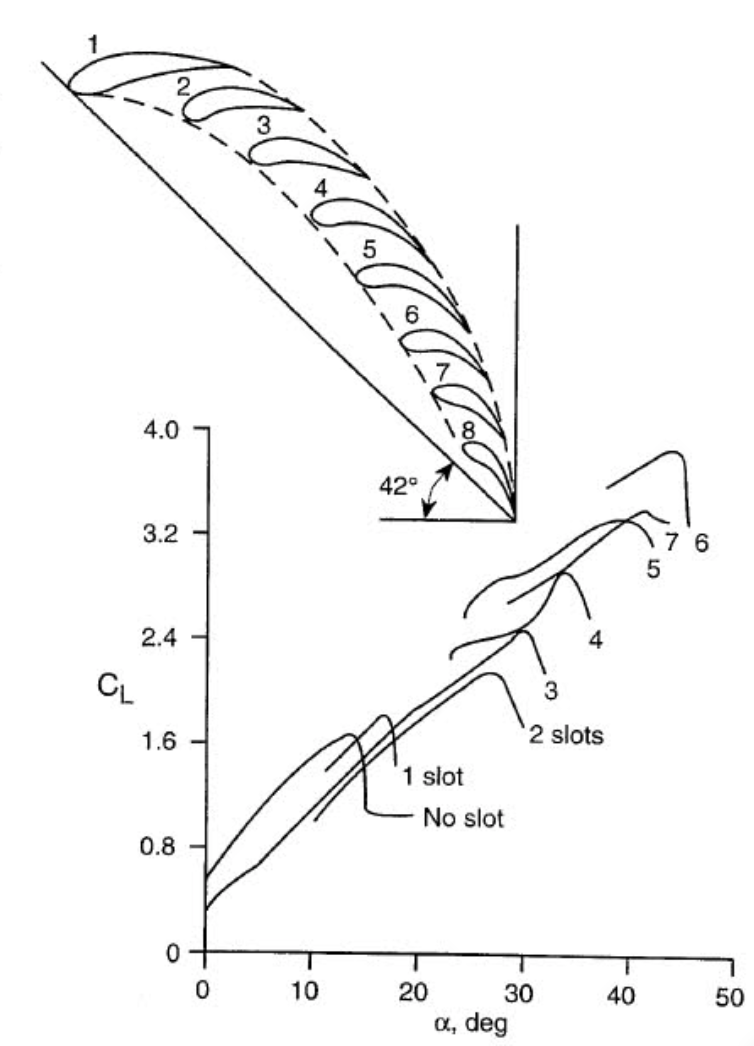
\includegraphics[width=\textwidth,rotate=1.5]{multielewing}
        \caption{Lift coefficient as a function of effective angle of attack. The \emph{No slot} line corresponds to a single element wing, and the \emph{1 slot} corresponds to a double element wing. Figure taken from \cite{jkatz}.}
        \label{fig:multielewing}
      \end{figure}

      As mentioned before, in order to increase downforce on a wing (made of a predefined airfoil) there is two options: Increasing the width of the wing, or increasing the camber. As the width is fixed by regulations, the camber has to be varied. Increasing camber usually causes flow separation, but by splitting the airfoil into multiple elements, this can be circumvented while gaining effective airfoil camber. The camber attained by using multiple elements is usually much higher than with a single element, and letting the high pressure from the first element transition to the low pressure zone of the secondary element results in a favorable interaction between the two elements \fxnote{is it this way that it works?}.

      The lift coefficient can be seen as a function of angle of attack in figure \ref{fig:multielewing}. Notice how the angle of attack can be increased before stalling occurs and lift increases. A leading airfoil (also called a \emph{slat}) will extend the angle of attack even further, but will not increase the lift curve \cite{jkatz}.

\section{Wing Parameters}

  The previous sections describe which parameters can be varied in order to attain better aerodynamical properties, such as higher lift, robustness towards stall and protection against trailing tip vortices. Improving a wing has several optimization parameters, and below is a table of how these are going to be handled in the following sections:
  \begin{table}
    \begin{tabularx}{\textwidth}[t]{>{\columncolor{seapurple!40}} l XX}
      \arrayrulecolor{seapurple}\hline
      \rowcolor{white}
      \textbf{\textcolor{seapurple}{Parameter}} & \textbf{\textcolor{seapurple}{Effect}} & \textbf{\textcolor{seapurple}{Optimization Technique}}\\
      \hline
      Thickness & Usually predefined by airfoil & N/A\\
      Angle of Attack & Changes lift characteristics & Finding the optimum angle of attack\\
      Camber & Usually predefined by airfoil & Adding additional Elements\\
      Position between elements & Changes lift characteristics & Optimizing $x,y$ position between elements\\
      Size & Sizes directly increases lift & Finding the maximum allowed size by regulations
    \end{tabularx}
    \caption{Table of parameters that can vary and how to optimize the parameter.}
  \end{table}
